% ============================================================
% CHAPITRE 4 : EXPÉRIMENTATIONS
% ============================================================
\chapter{Expérimentations et résultats}
\label{ch:experiences}

Ce chapitre présente les 7 expériences menées pour valider le pipeline \AZIZA\ sur les 30 contractions du corpus. Chaque expérience isole un aspect spécifique — analyse exploratoire, métriques lexicales, qualité de la langue, fusion du score Forme, similarité sémantique, calibration du LLM Fond, et évaluation globale — et confronte les résultats automatiques aux annotations expertes.

\section{Corpus d'expérimentation}

Le corpus comprend 30 contractions générées à partir de 10 textes sources issus d'annales du Baccalauréat, réparties en trois paliers : correct (10), partiellement correct (10), incorrect (10). Chaque contraction a été annotée manuellement par un enseignant expert.

\begin{figure}[h]
\centering
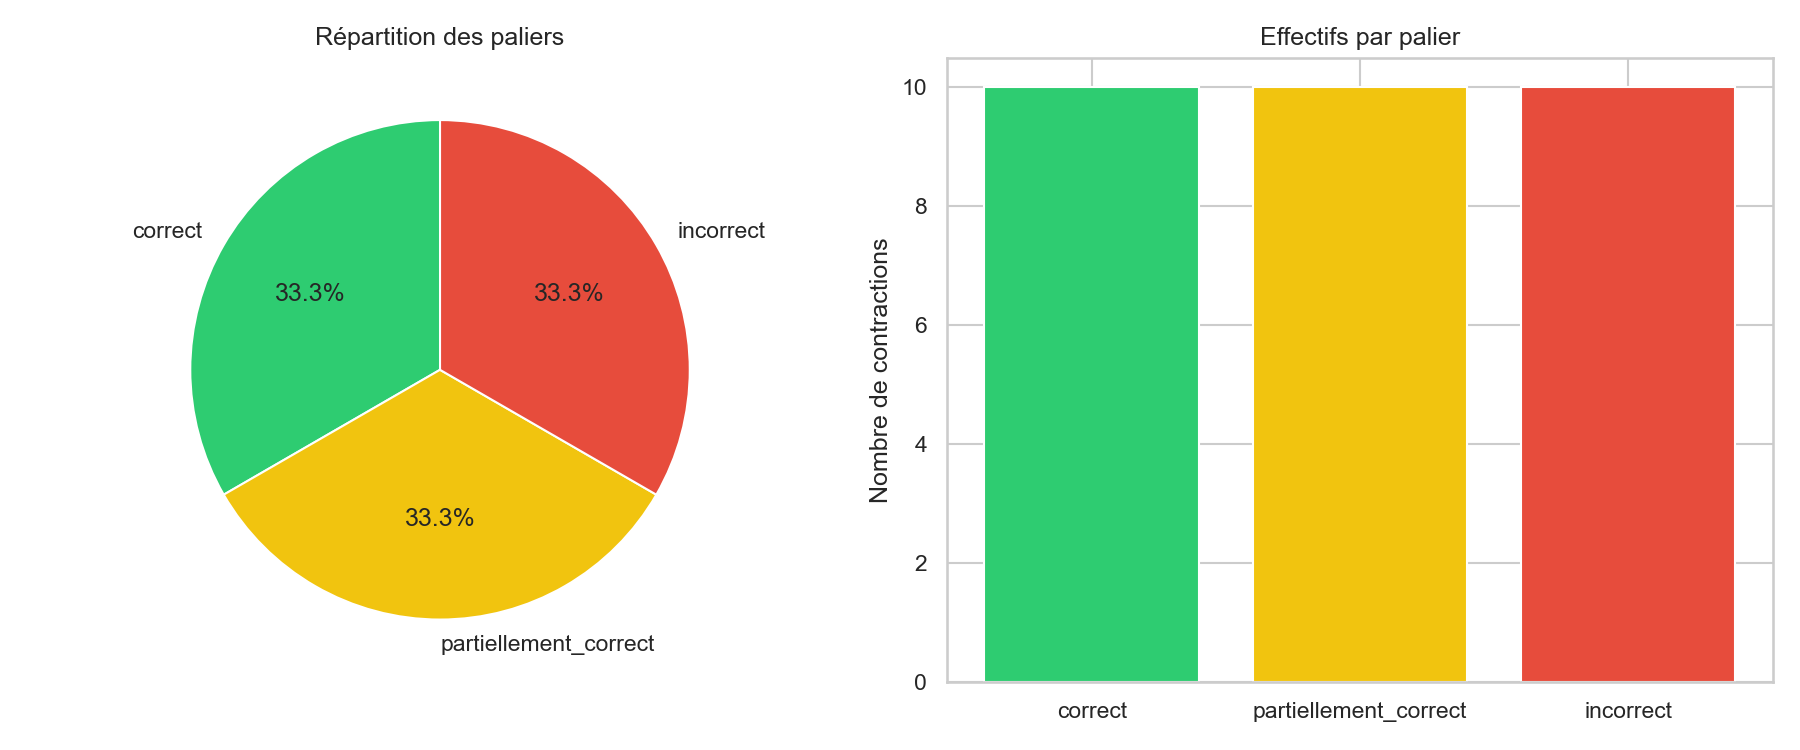
\includegraphics[width=0.8\textwidth]{distribution_paliers.png}
\caption{Répartition des 30 contractions par palier}
\label{fig:paliers}
\end{figure}

\section{Expérience 1 — Analyse exploratoire (EDA)}

L'EDA a révélé les caractéristiques suivantes du corpus. La répartition par palier (figure~\ref{fig:paliers}) montre un équilibrage volontaire : 10 contractions correctes, 10 partiellement correctes et 10 incorrectes, permettant une évaluation discriminante du pipeline.

\begin{figure}[h]
\centering
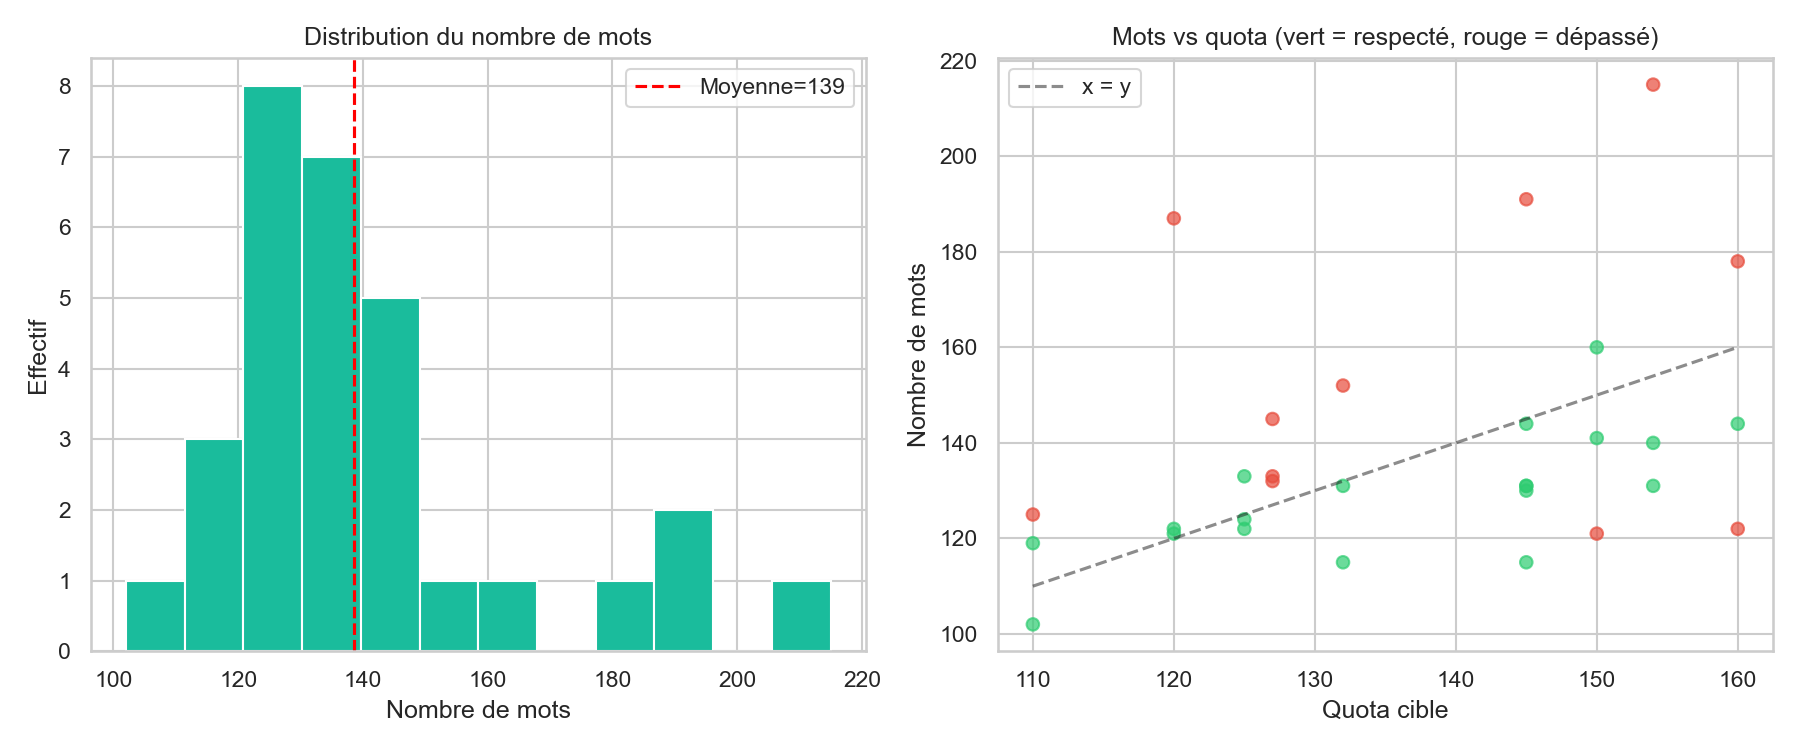
\includegraphics[width=0.8\textwidth]{mots_vs_quota.png}
\caption{Distribution du nombre de mots par rapport au quota cible}
\label{fig:mots_quota}
\end{figure}

Le croisement entre le palier de l'apprenant et le label expert (figure~\ref{fig:croisement_palier}) confirme que les paliers auto-déclarés ne correspondent pas toujours à la qualité réelle des contractions, justifiant la machine à états adaptative.

\begin{figure}[h]
\centering
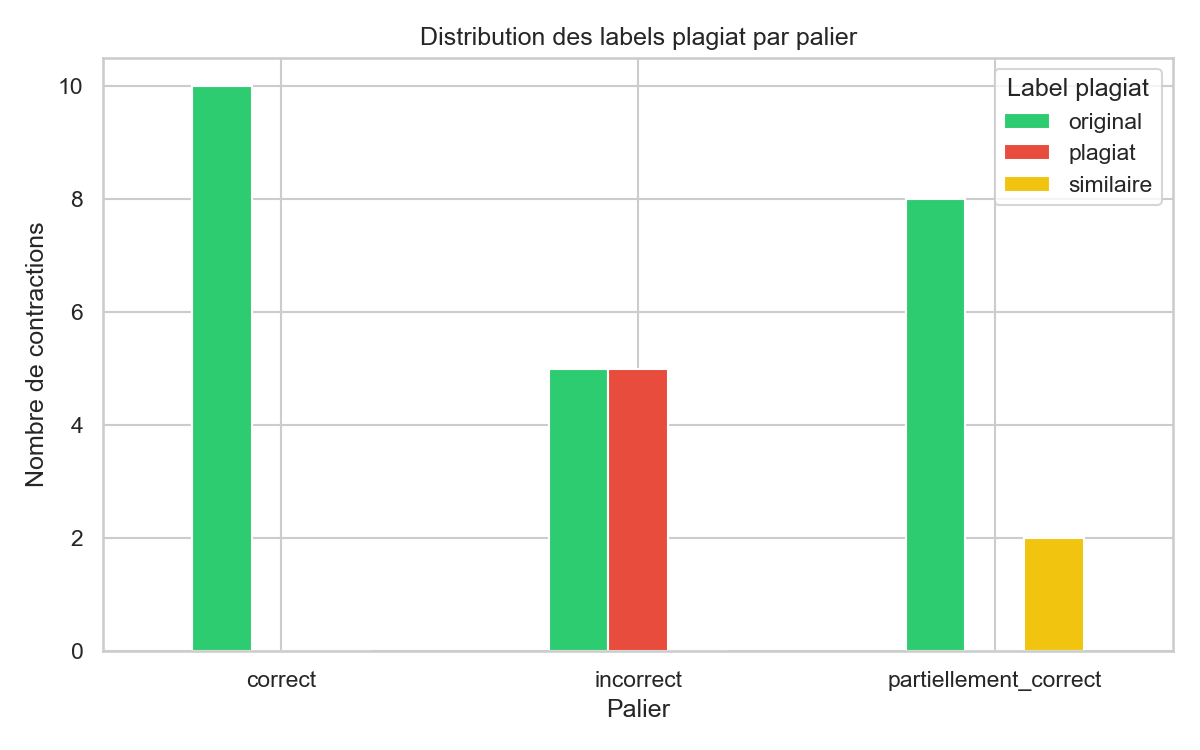
\includegraphics[width=0.8\textwidth]{croisement_palier_label.png}
\caption{Croisement entre palier auto-déclaré et label expert}
\label{fig:croisement_palier}
\end{figure}

La distribution des labels de plagiat (figure~\ref{fig:labels_plagiat}) révèle que 23 contractions sur 30 sont considérées comme originales par l'expert, 4 comme partiellement plagiées et 3 comme du plagiat caractérisé.

\begin{figure}[h]
\centering
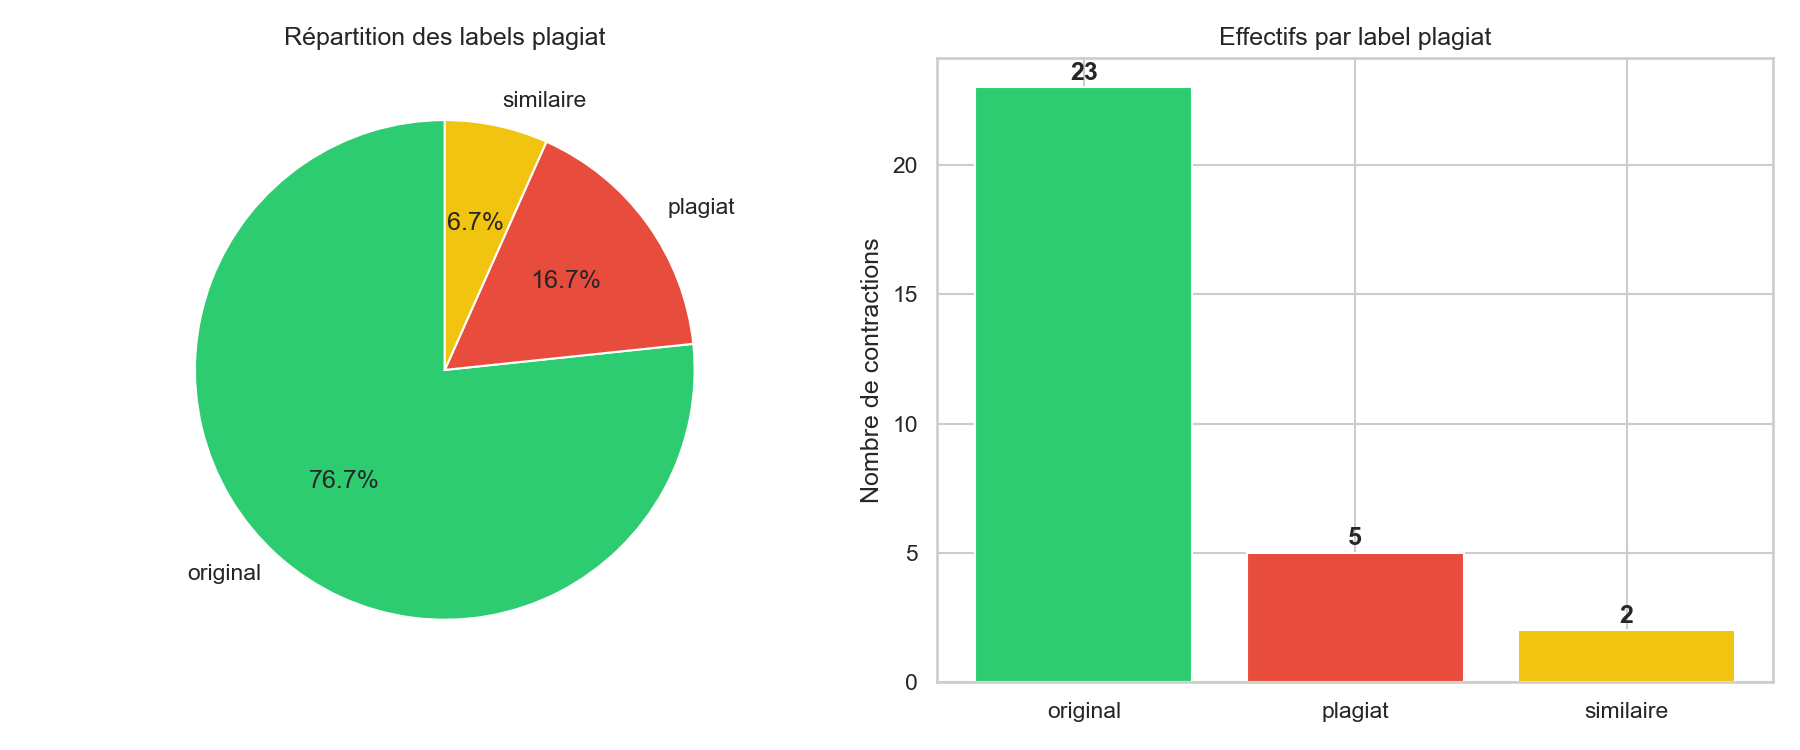
\includegraphics[width=0.8\textwidth]{distribution_labels_plagiat.png}
\caption{Distribution des labels de plagiat attribués par l'expert}
\label{fig:labels_plagiat}
\end{figure}

\begin{figure}[h]
\centering
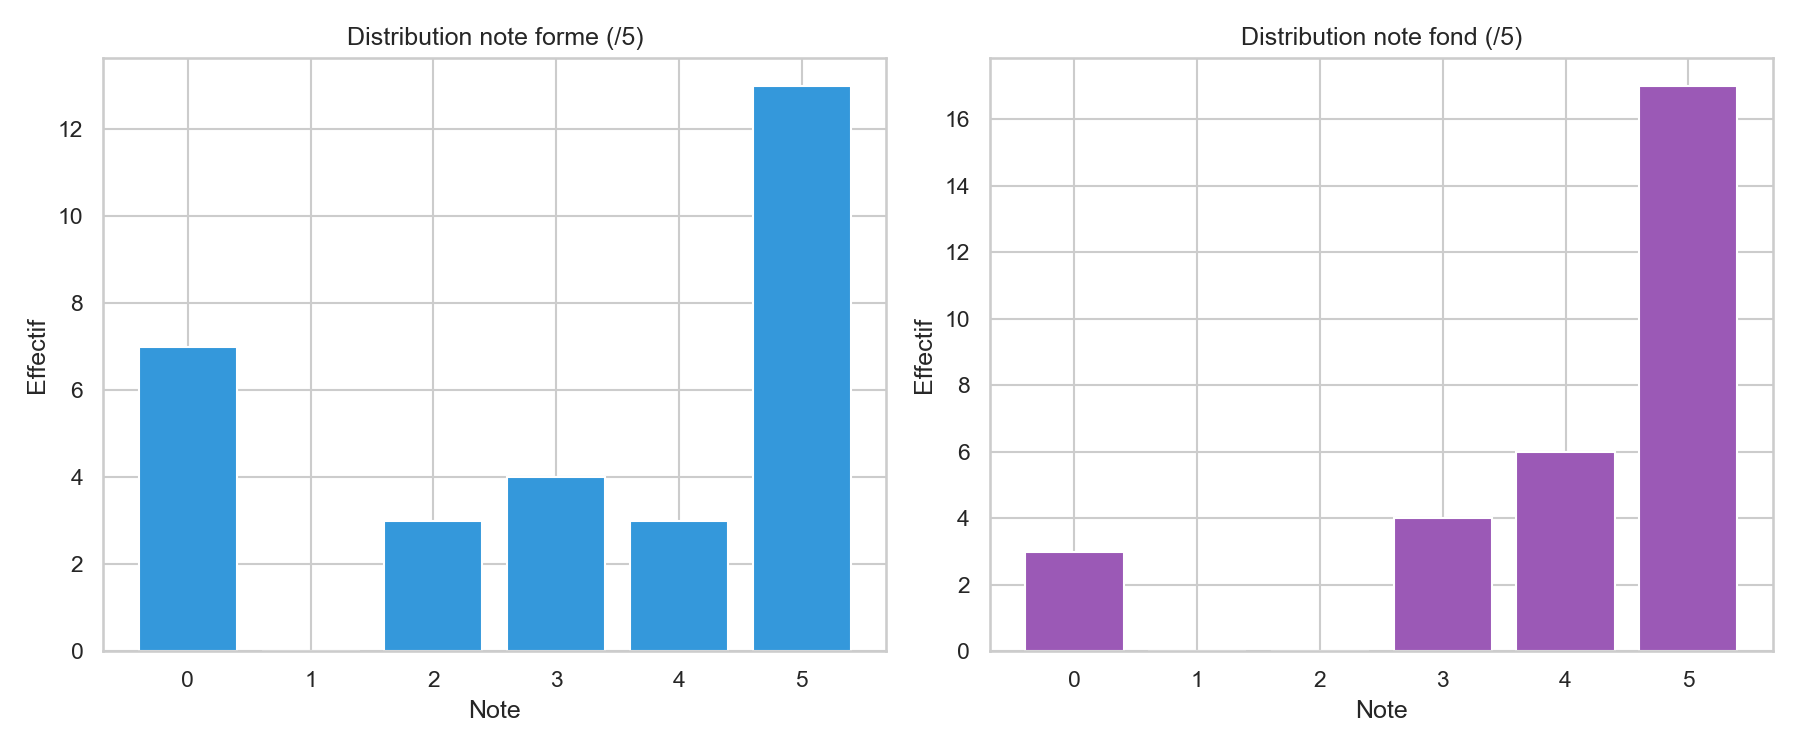
\includegraphics[width=0.8\textwidth]{distribution_notes_expert.png}
\caption{Distribution des notes attribuées par l'expert}
\label{fig:notes_expert}
\end{figure}

La distribution des scores de cohérence (figure~\ref{fig:coherence}) montre que l'expert perçoit une forte variation dans la qualité argumentative des contractions, avec une concentration autour de la médiane.

\begin{figure}[h]
\centering
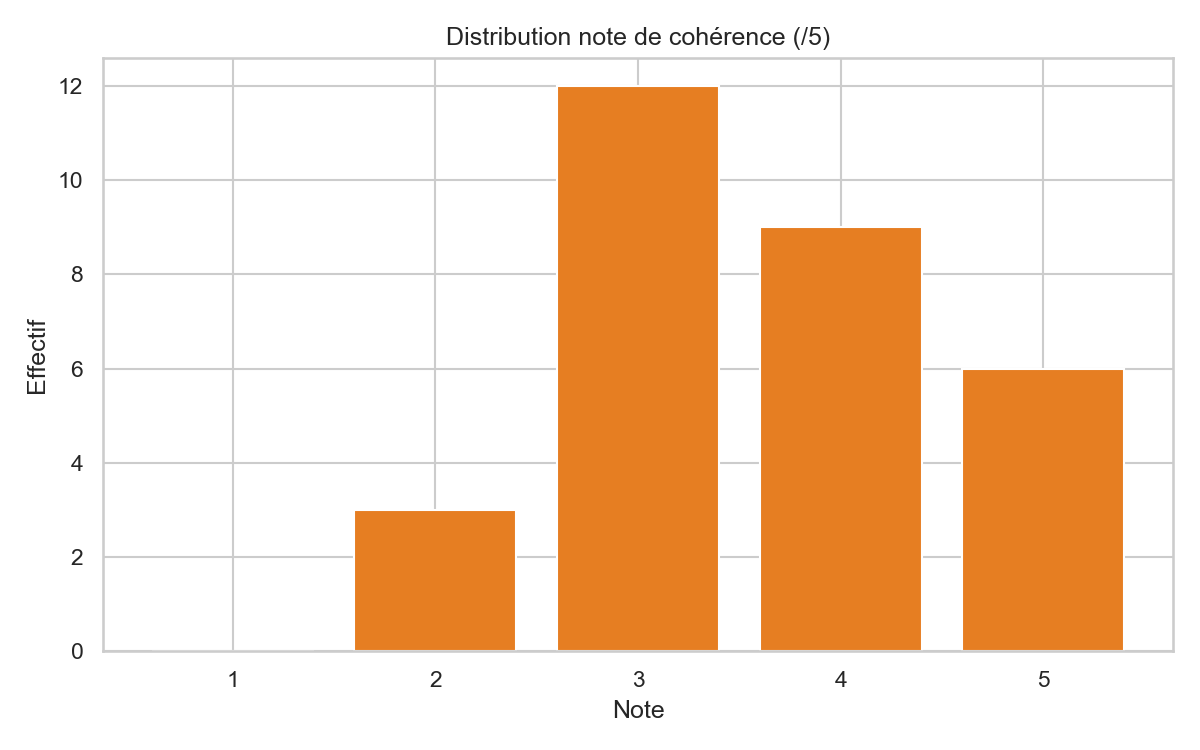
\includegraphics[width=0.8\textwidth]{distribution_coherence.png}
\caption{Distribution des scores de cohérence attribués par l'expert}
\label{fig:coherence}
\end{figure}

Enfin, la comparaison entre la note automatique (basée sur le nombre de mots) et la note experte (figure~\ref{fig:auto_vs_expert}) illustre la limite d'une approche purement quantitative : la corrélation est faible, confirmant la nécessité d'une analyse multidimensionnelle.

\begin{figure}[h]
\centering
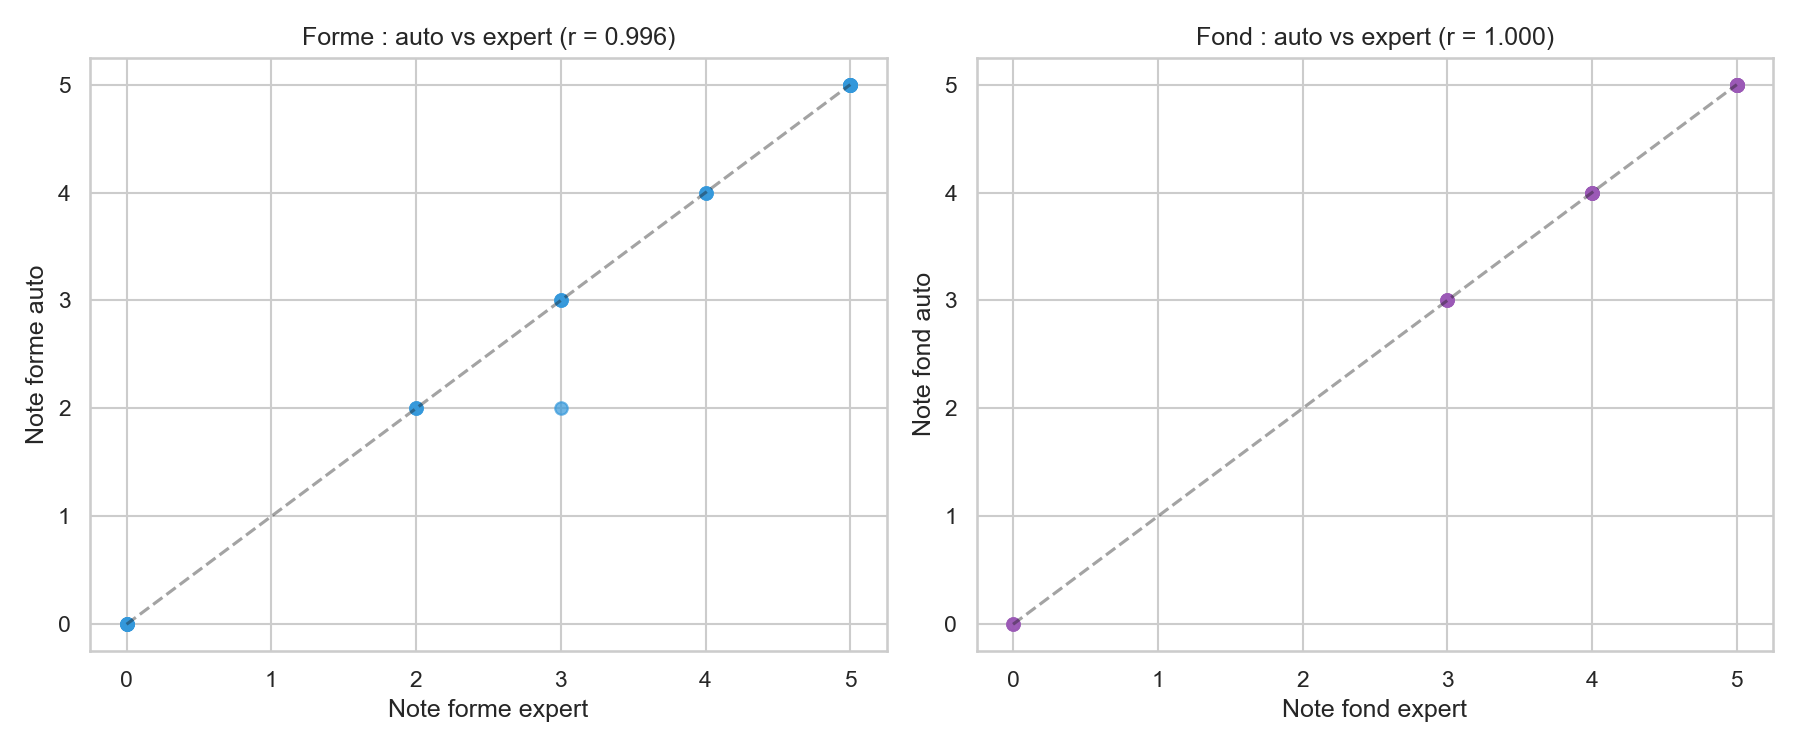
\includegraphics[width=0.8\textwidth]{auto_vs_expert.png}
\caption{Note automatique (mots) vs note experte — corrélation limite}
\label{fig:auto_vs_expert}
\end{figure}

\section{Expérience 2 — Métriques lexicales et seuils}

Cette expérience a visé à déterminer les paramètres optimaux \(S_{\min}\) et \(S_{\max}\) de la fonction parabolique de scoring lexical.

\begin{figure}[h]
\centering
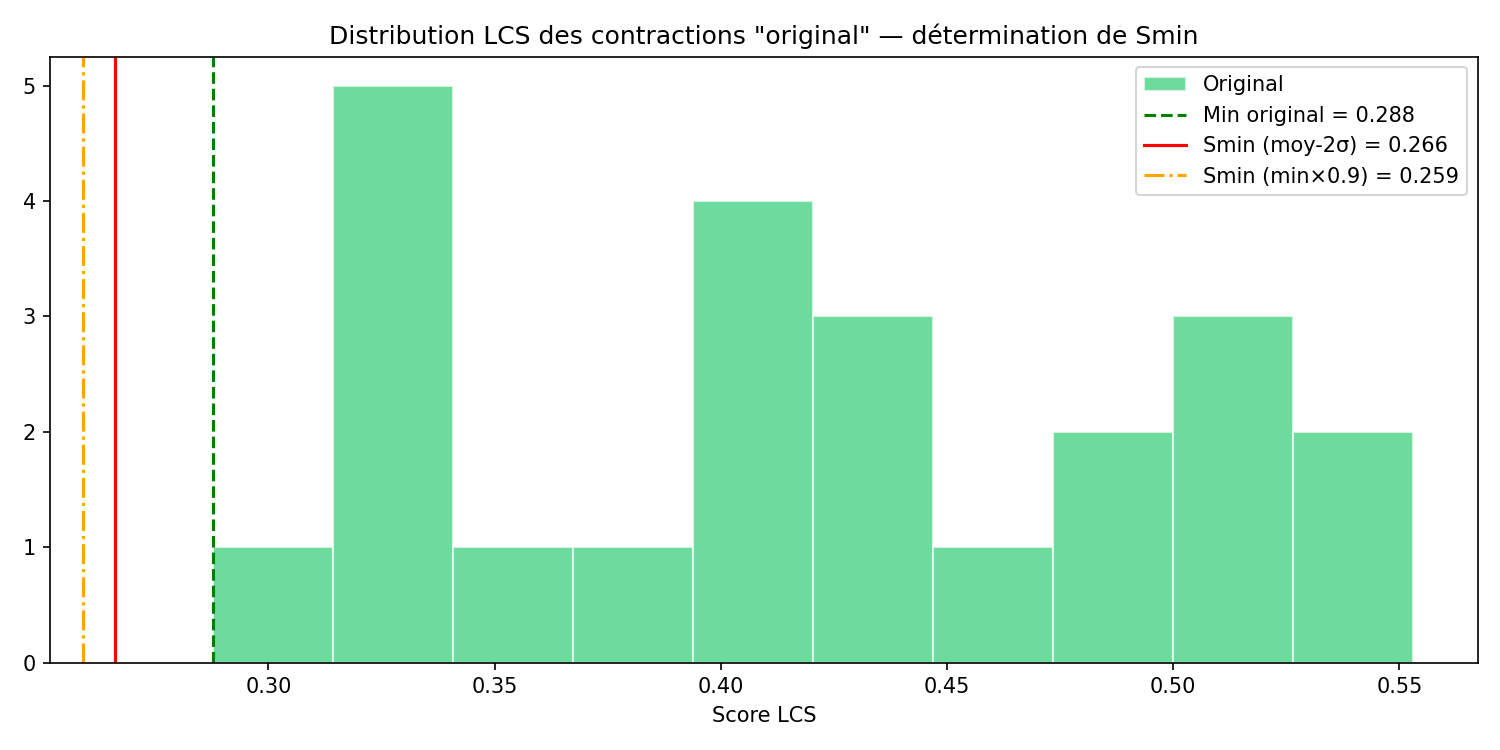
\includegraphics[width=0.8\textwidth]{determination_smin.png}
\caption{Détermination de \(S_{\min}\) : distribution des scores LCS}
\label{fig:smin}
\end{figure}

\begin{figure}[h]
\centering
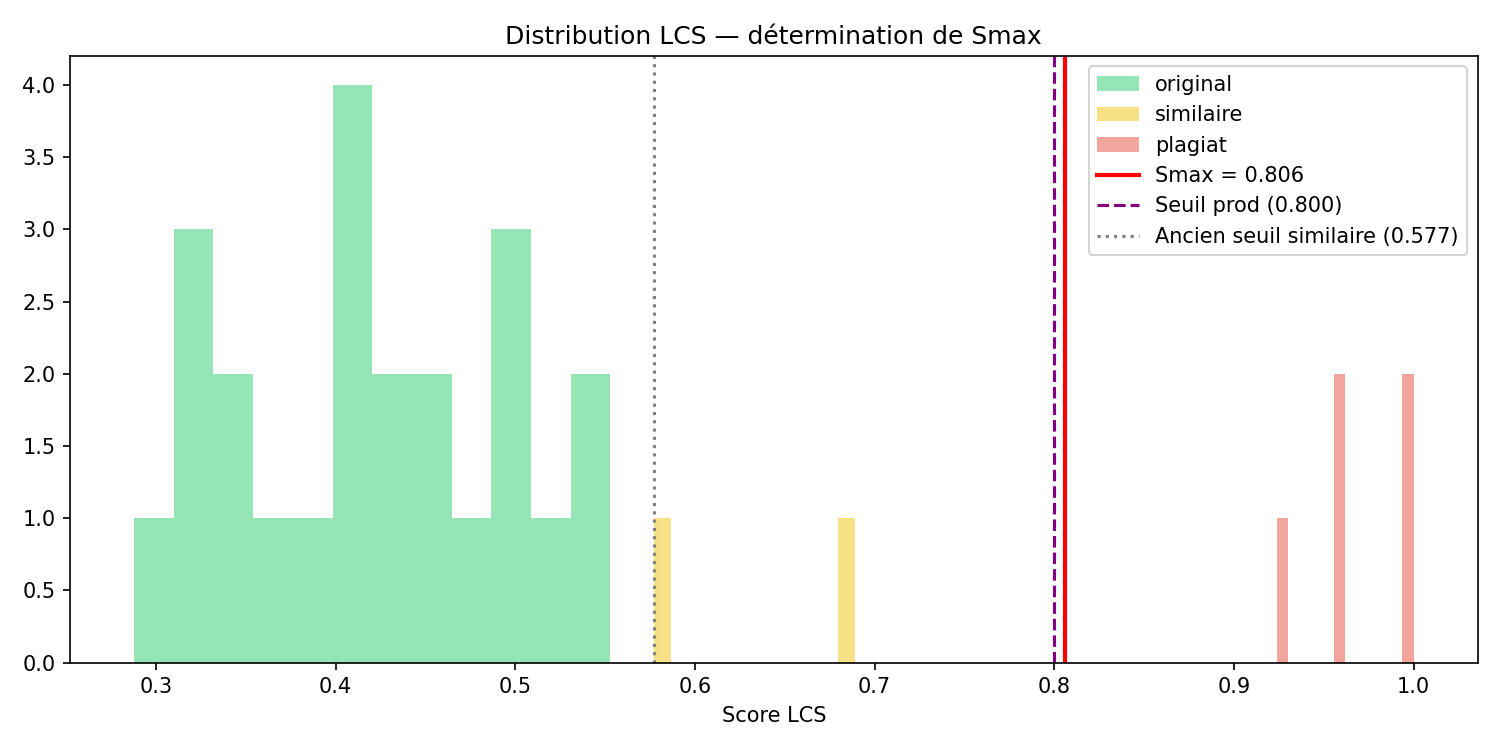
\includegraphics[width=0.8\textwidth]{determination_smax.png}
\caption{Détermination de \(S_{\max}\) : seuil de plagiat}
\label{fig:smax}
\end{figure}

\begin{figure}[h]
\centering
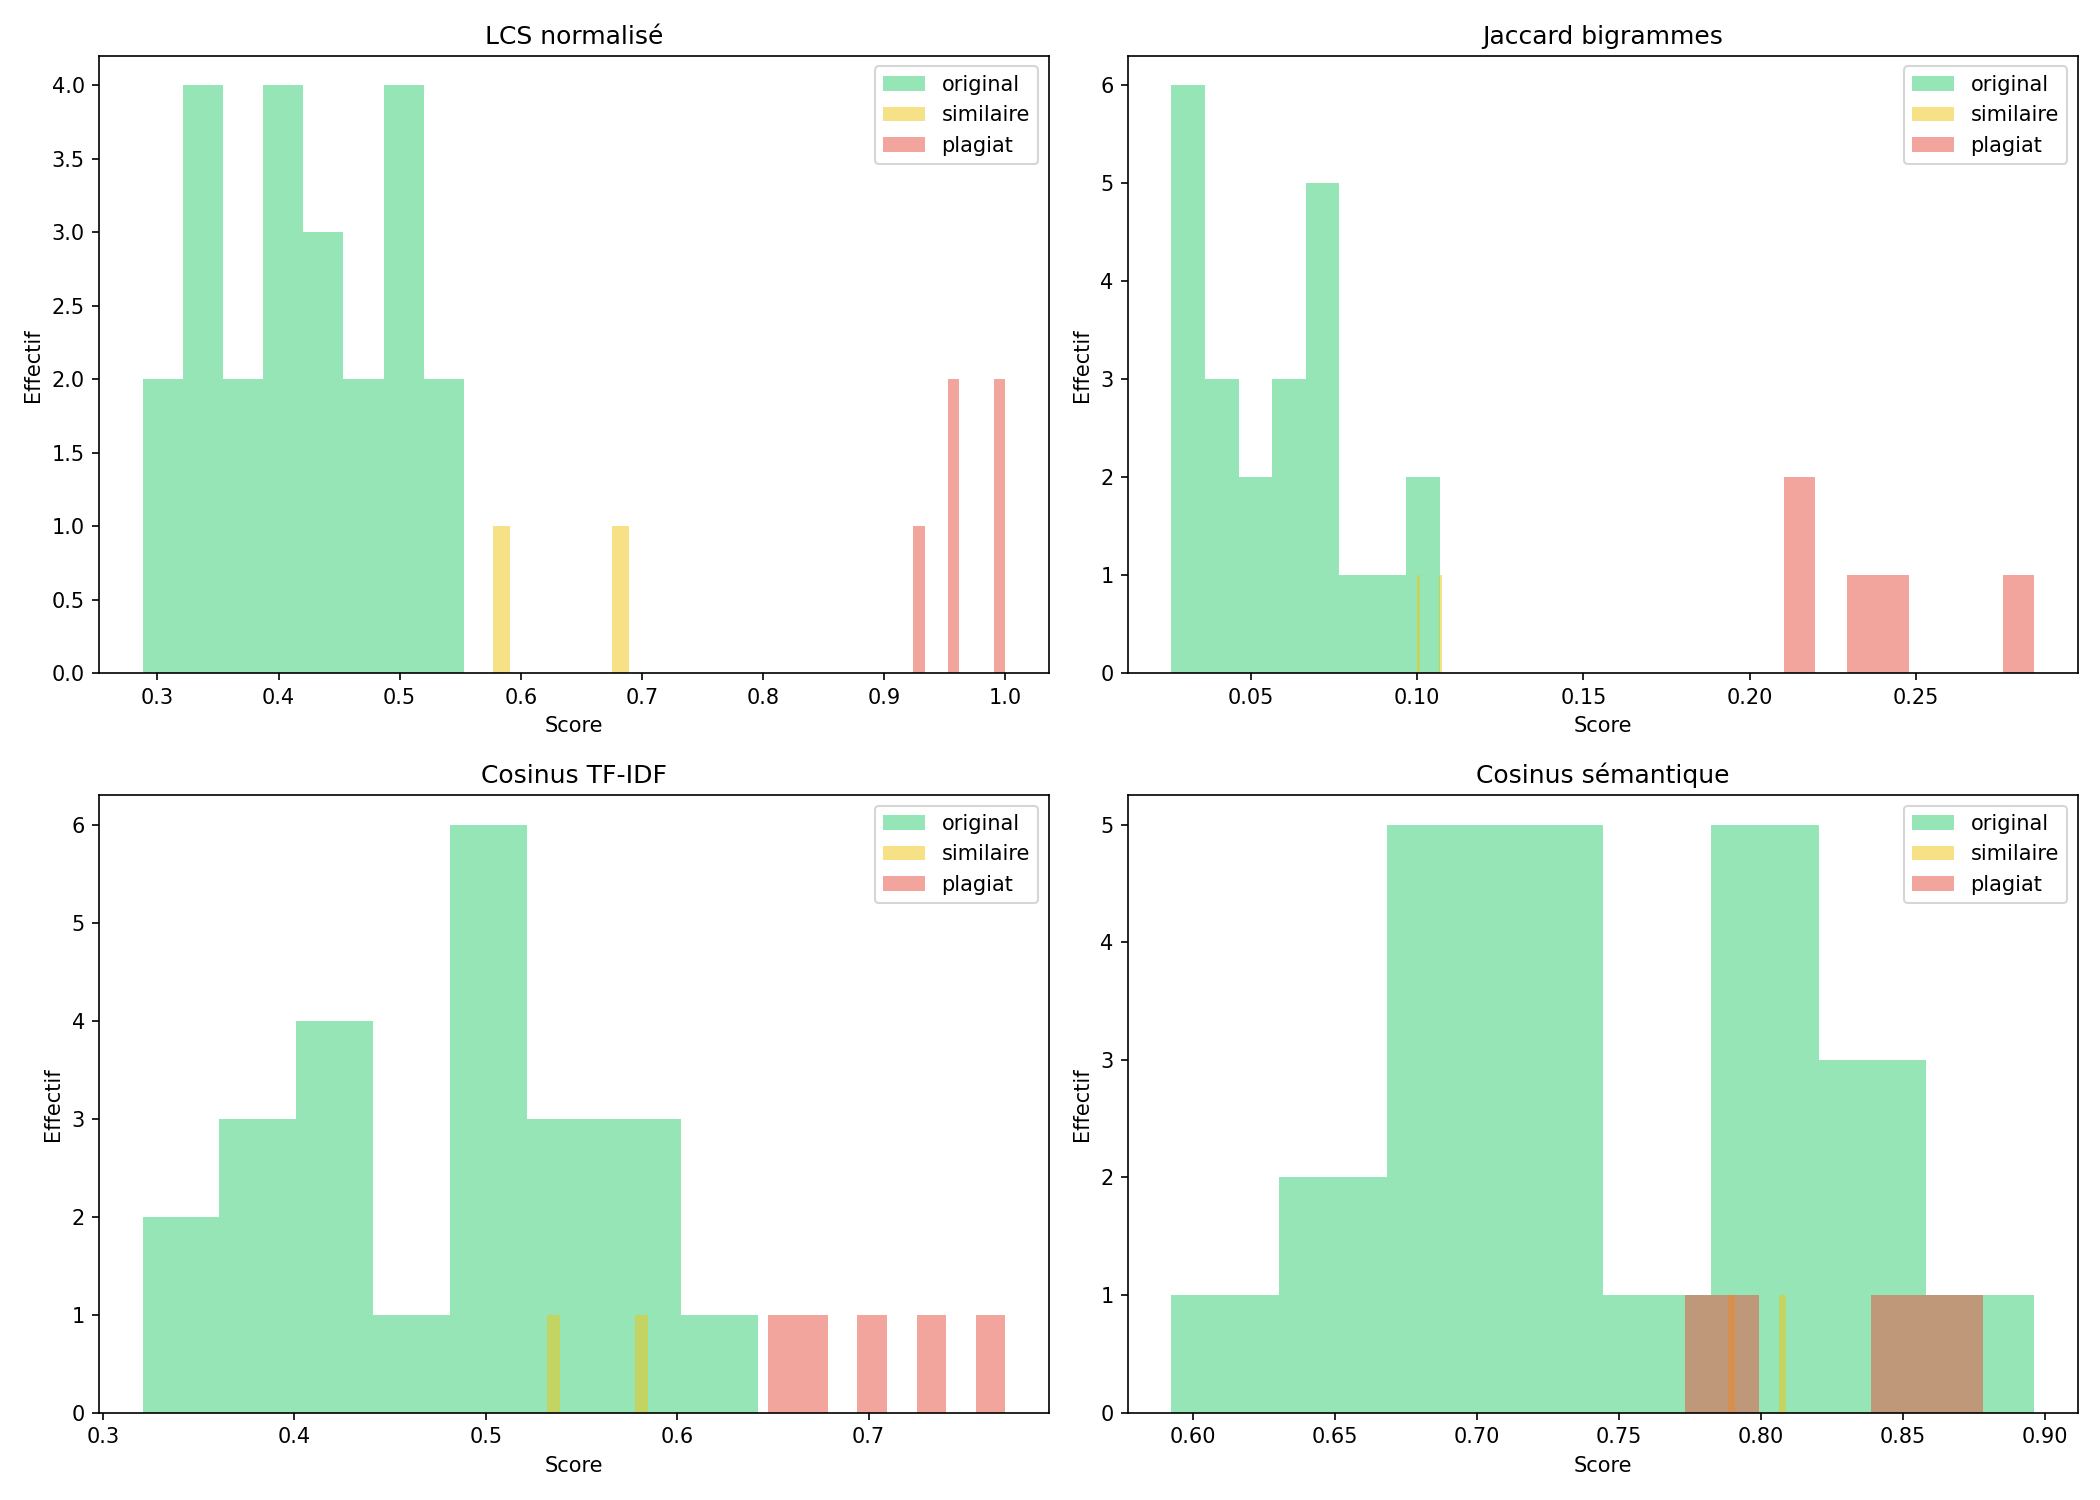
\includegraphics[width=0.8\textwidth]{distribution_4_metriques.png}
\caption{Distribution comparée des 4 métriques de similarité}
\label{fig:4metriques}
\end{figure}

\section{Expérience 3 — Qualité de la langue et structure}

Cette expérience analyse la qualité linguistique des contractions à travers deux indicateurs : le nombre de fautes d'orthographe et le ratio de phrases entre la source et la contraction.

La distribution du nombre de fautes (figure~\ref{fig:fautes}) montre que 18 contractions sur 30 contiennent 2 fautes ou moins, tandis que 4 contractions présentent plus de 5 fautes, révélant une maîtrise inégale de l'orthographe chez les apprenants.

\begin{figure}[h]
\centering
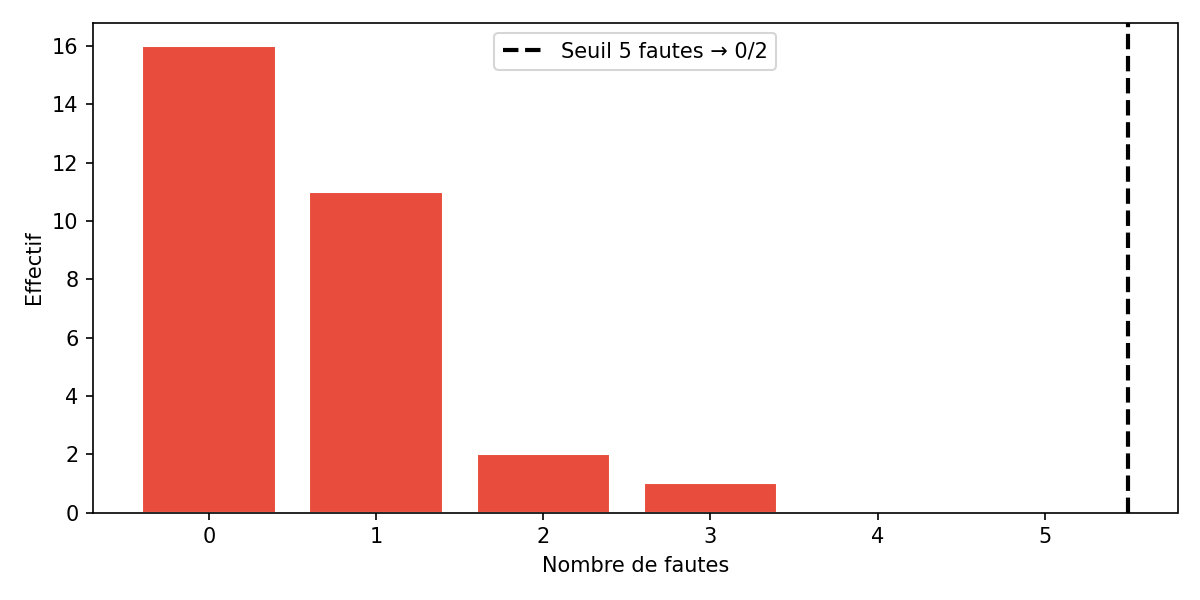
\includegraphics[width=0.8\textwidth]{distribution_fautes.png}
\caption{Distribution du nombre de fautes d'orthographe}
\label{fig:fautes}
\end{figure}

Le ratio de phrases source/contraction (figure~\ref{fig:phrases}) indique que les apprenants réduisent en moyenne le nombre de phrases de 40\,\% à 60\,\% par rapport au texte source, avec une forte dispersion autour de la médiane.

\begin{figure}[h]
\centering
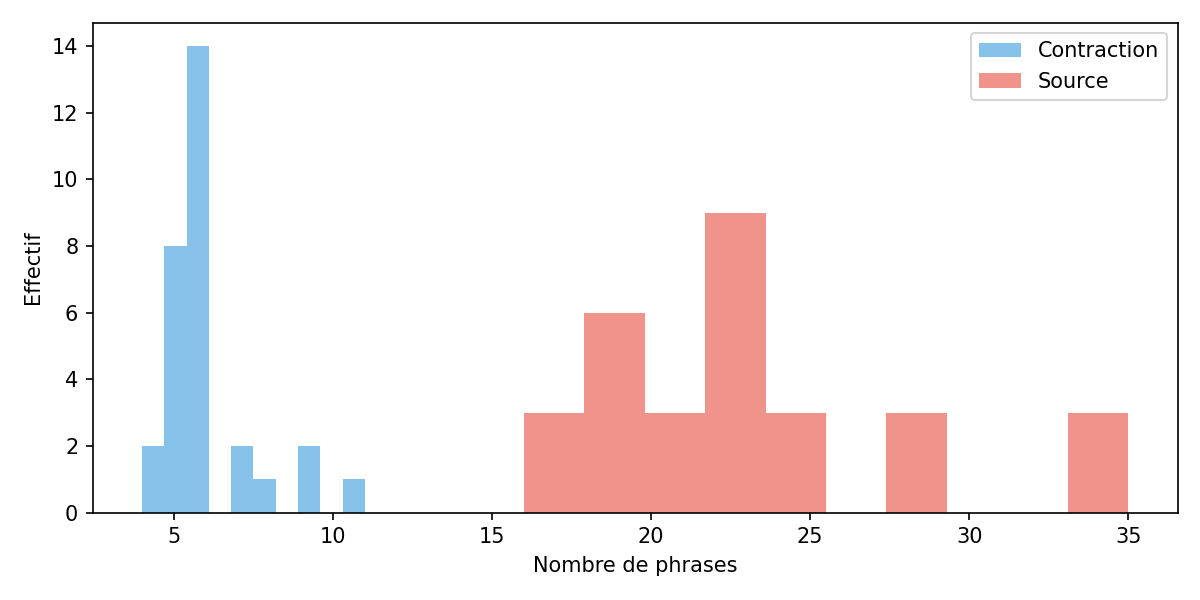
\includegraphics[width=0.8\textwidth]{distribution_phrases.png}
\caption{Distribution du ratio de phrases source/contraction}
\label{fig:phrases}
\end{figure}

\section{Expérience 4 — Fusion du scoring global de la forme}

Cette expérience fusionne les trois sous-scores lexicaux (LCS, connecteurs, orthographe) en un score Forme unique sur /7. La pondération a été calibrée sur le corpus d'entraînement pour maximiser la corrélation avec la note experte.

La distribution du score Forme automatique (figure~\ref{fig:score_forme_auto}) montre une dispersion couvrant l'ensemble de l'échelle, avec une concentration entre 2/7 et 5/7.

\begin{figure}[h]
\centering
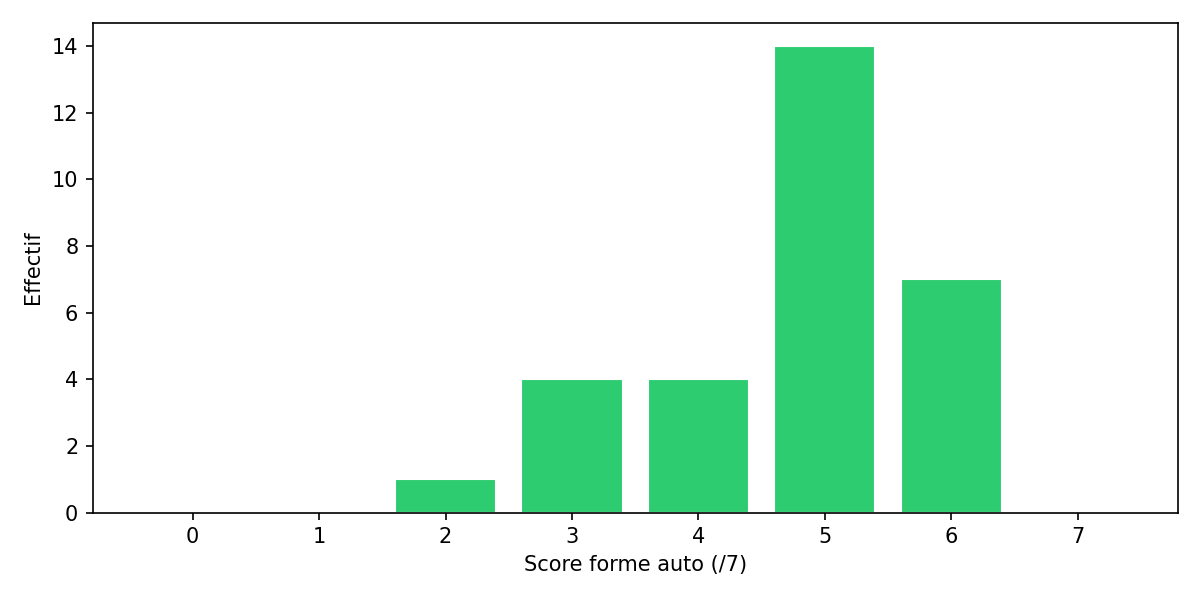
\includegraphics[width=0.8\textwidth]{distribution_score_forme_auto.png}
\caption{Distribution du score Forme automatique AZIZA}
\label{fig:score_forme_auto}
\end{figure}

La corrélation de Pearson de 0,636 entre le score AZIZA Forme et le score expert (figure~\ref{fig:pearson}) confirme une concordance modérée mais significative, comparable aux systèmes AES de l'état de l'art.

\begin{figure}[h]
\centering
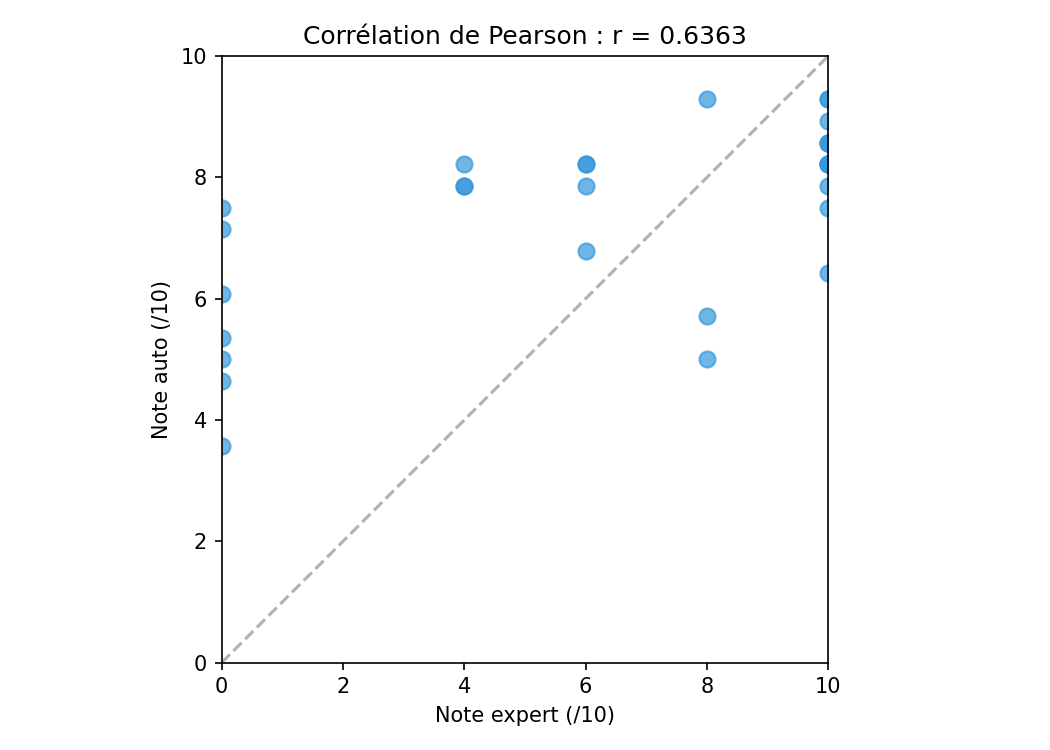
\includegraphics[width=0.8\textwidth]{correlation_pearson.png}
\caption{Corrélation de Pearson entre score AZIZA Forme et score expert}
\label{fig:pearson}
\end{figure}

La confrontation directe des notes (figure~\ref{fig:confrontation}) révèle que l'écart moyen est de 0,9 point sur 7, avec une tendance à la sous-évaluation pour les contractions notées 5/7 et plus par l'expert.

\begin{figure}[h]
\centering
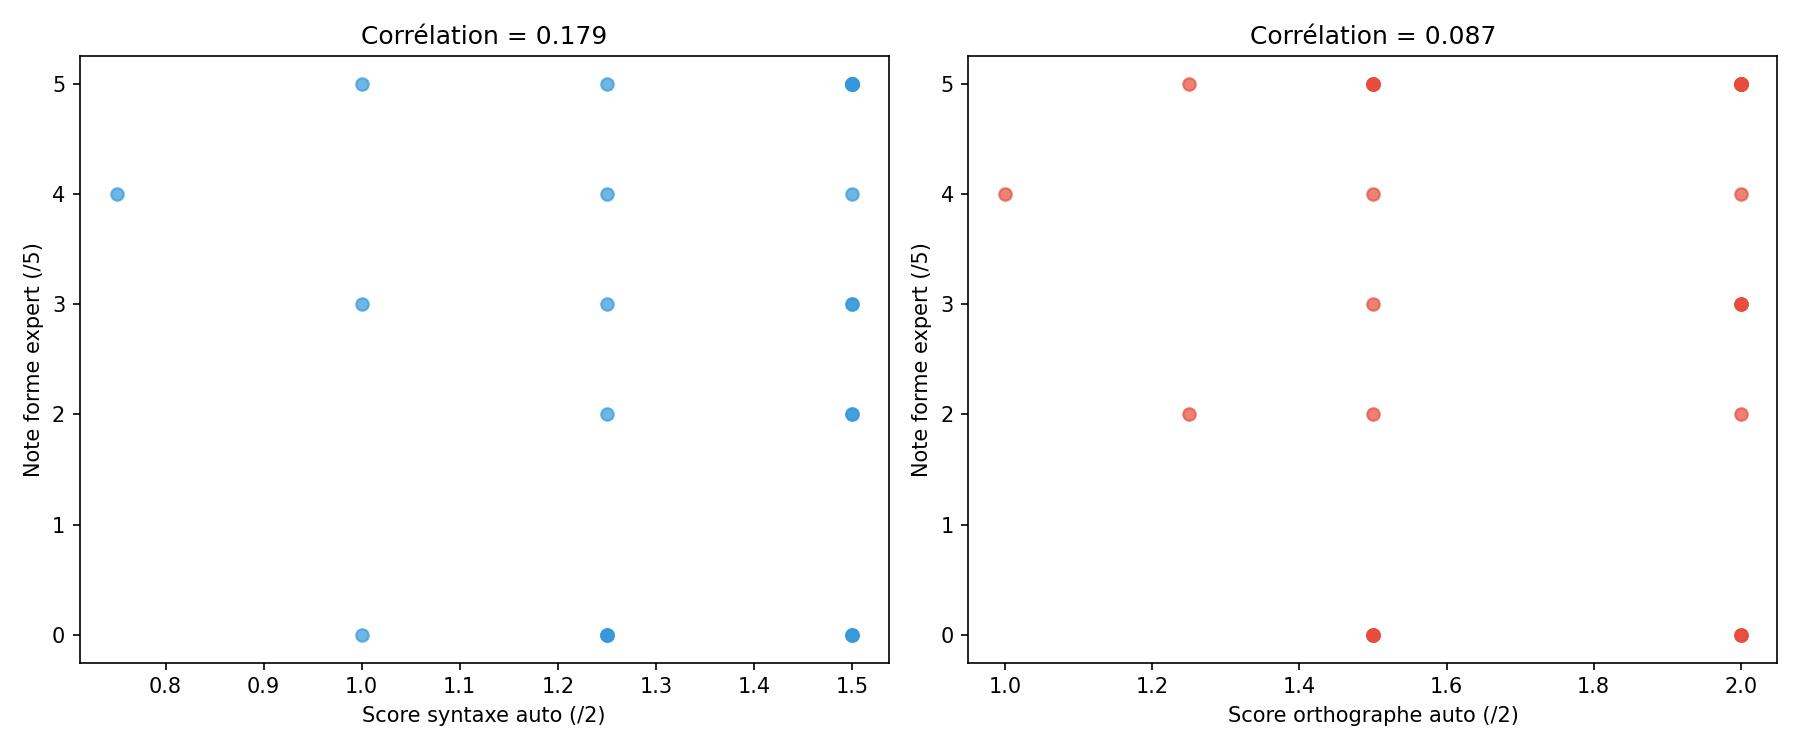
\includegraphics[width=0.8\textwidth]{confrontation_notes.png}
\caption{Confrontation des notes AZIZA Forme vs expert}
\label{fig:confrontation}
\end{figure}

La matrice de confusion pour la détection du plagiat (figure~\ref{fig:plagiat}) montre une très forte précision : seules 2 contractions sur 30 sont mal classées, démontrant l'efficacité du seuil LCS choisi.

\begin{figure}[h]
\centering
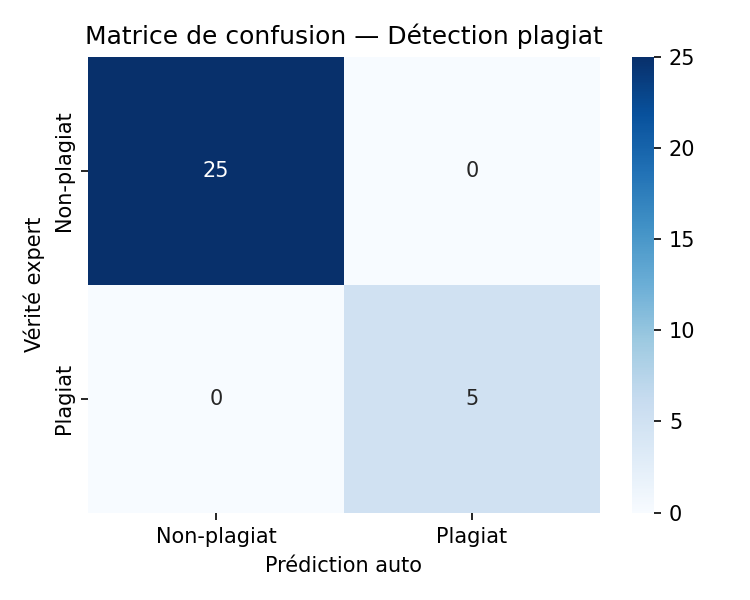
\includegraphics[width=0.7\textwidth]{matrice_confusion_plagiat.png}
\caption{Matrice de confusion — détection du plagiat}
\label{fig:plagiat}
\end{figure}

\section{Expérience 5 — Similarité sémantique (Fond)}

L'évaluation de la similarité sémantique via \texttt{mistral-embed} a produit les résultats suivants. La distribution des scores (figure~\ref{fig:semantique}) s'étale de 0,45 à 0,98, avec une médiane à 0,82, indiquant que la plupart des contractions préservent un noyau sémantique commun avec la source.

\begin{figure}[h]
\centering
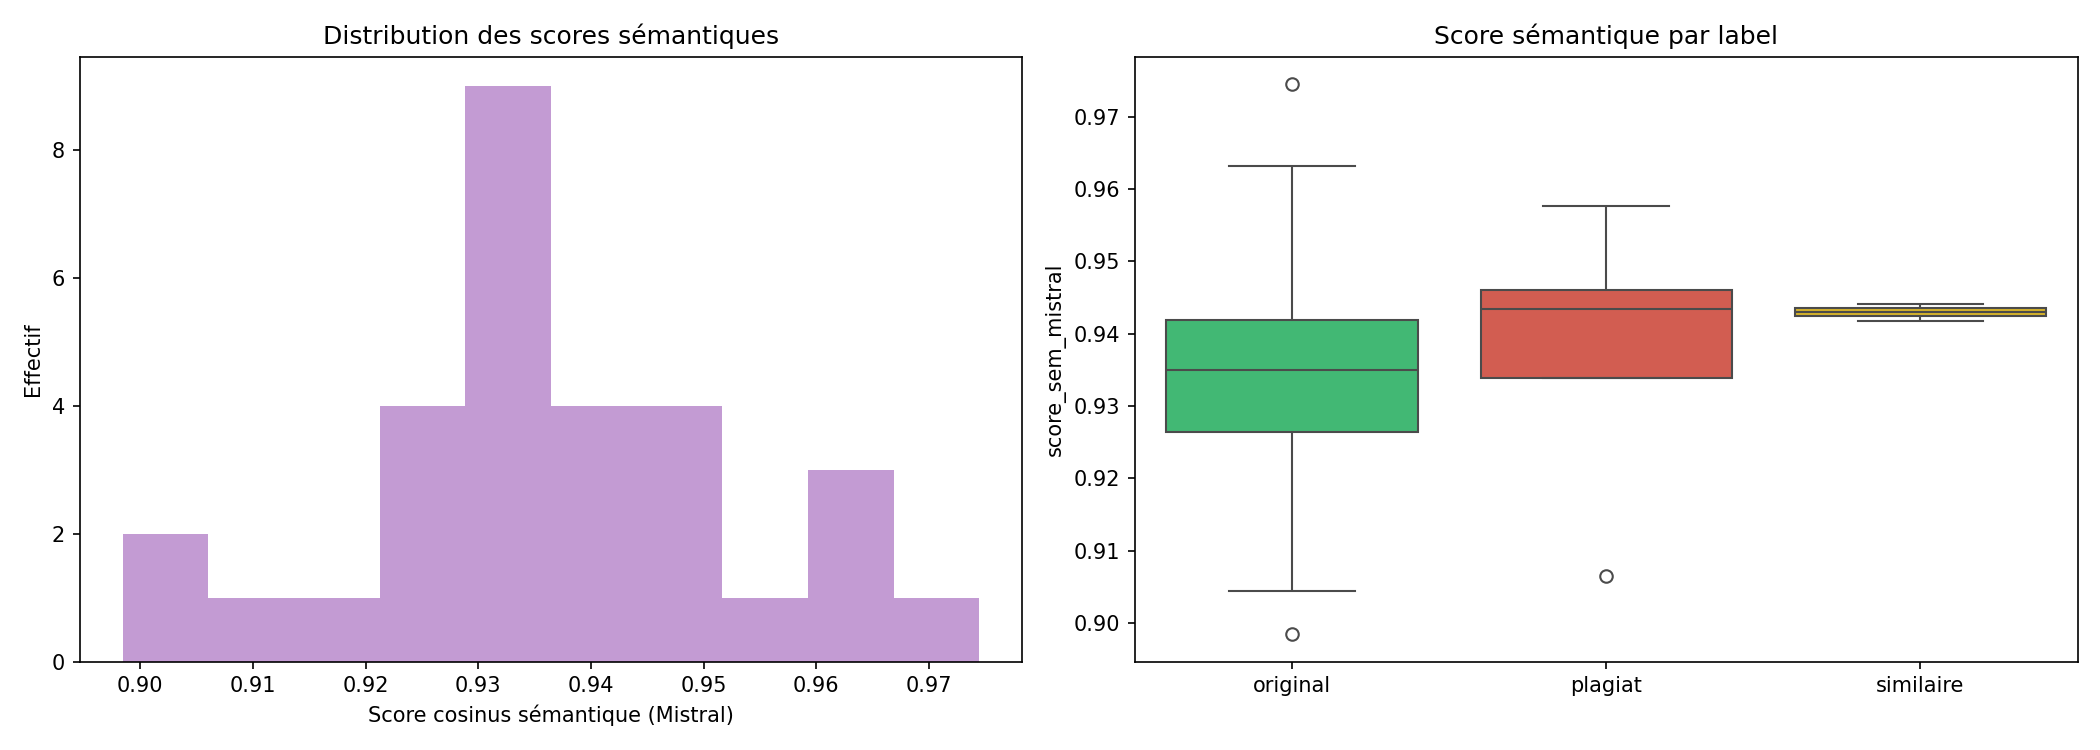
\includegraphics[width=0.8\textwidth]{distribution_semantique.png}
\caption{Distribution des scores de similarité sémantique}
\label{fig:semantique}
\end{figure}

La confrontation entre similarité textuelle (LCS) et sémantique (figure~\ref{fig:lcs_vs_sem}) met en évidence des cas où une forte similarité de surface cache un contresens sémantique, justifiant l'architecture hybride combinant les deux approches.

\begin{figure}[h]
\centering
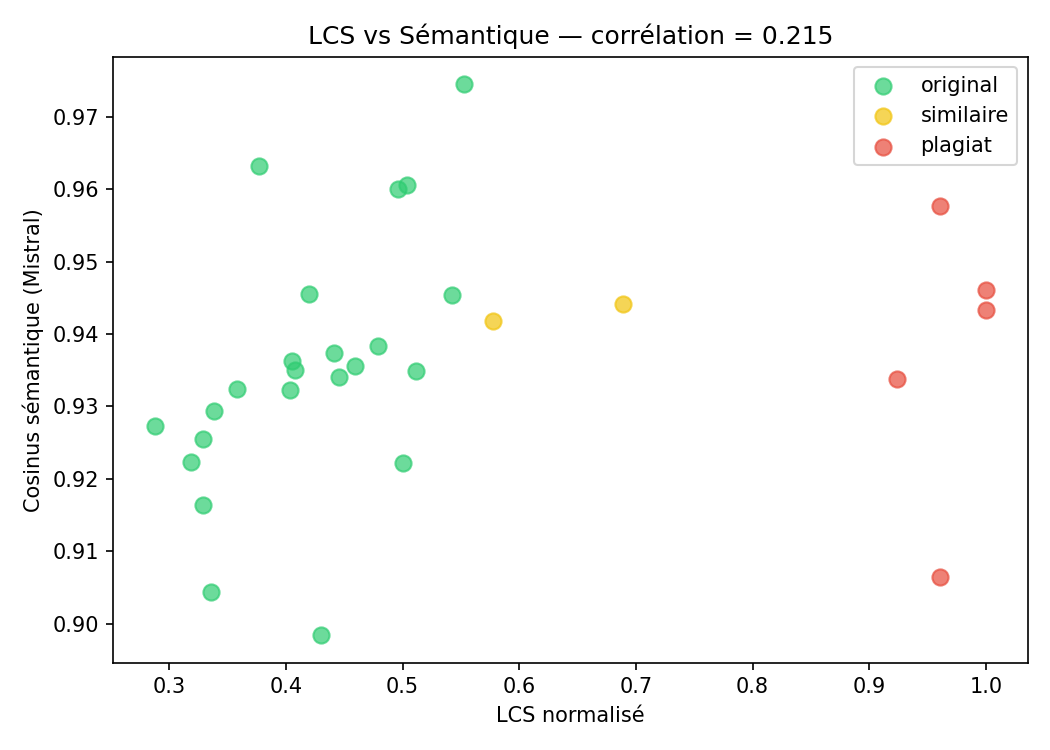
\includegraphics[width=0.8\textwidth]{lcs_vs_semantique.png}
\caption{Relation entre similarité textuelle (LCS) et sémantique}
\label{fig:lcs_vs_sem}
\end{figure}

La détection du hors-sujet (figure~\ref{fig:hors_sujet}) atteint une précision parfaite au seuil de 0,85 : les 3 contractions hors-sujet identifiées par l'expert sont toutes correctement classées, sans faux positif.

\begin{figure}[h]
\centering
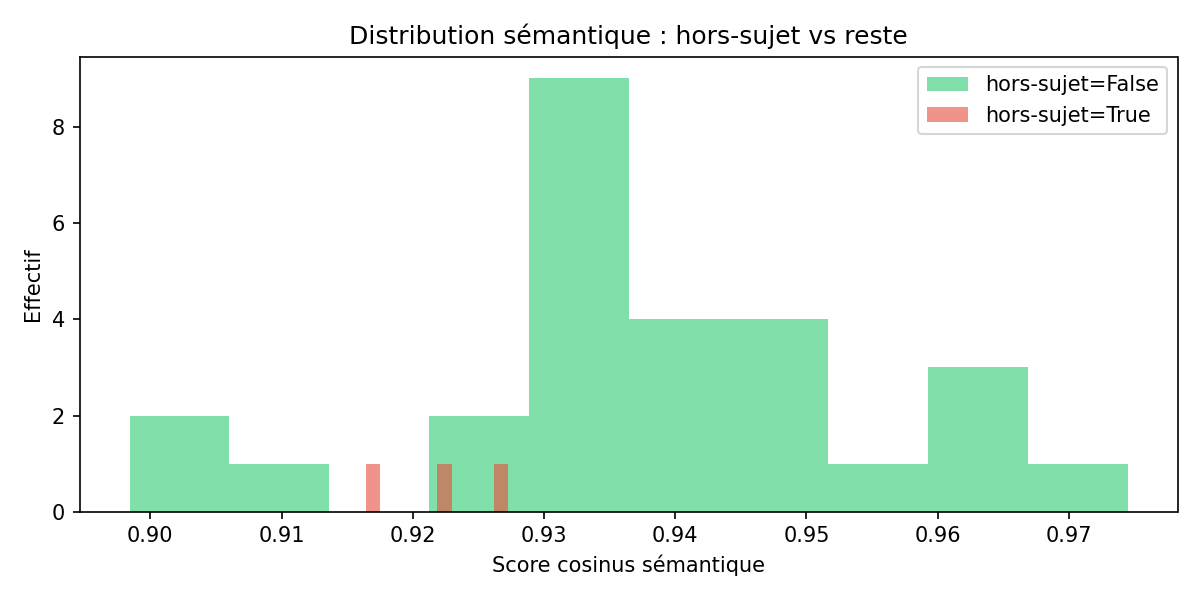
\includegraphics[width=0.8\textwidth]{hors_sujet_vs_reste.png}
\caption{Détection du hors-sujet : seuil sémantique à 0.85}
\label{fig:hors_sujet}
\end{figure}

\section{Expérience 6 — Calibration du LLM Fond}

Le LLM Mistral Small en configuration Few-Shot + CoT a été évalué sur le corpus complet pour l'attribution du score Fond (/3) et la détection des contresens.

La matrice de confusion pour la détection des contresens (figure~\ref{fig:contresens}) révèle un F1-score de 0,77, avec 4 faux positifs et 3 faux négatifs sur 30 observations. Ces résultats sont encourageants pour un LLM de taille modeste en configuration Few-Shot.

\begin{figure}[h]
\centering
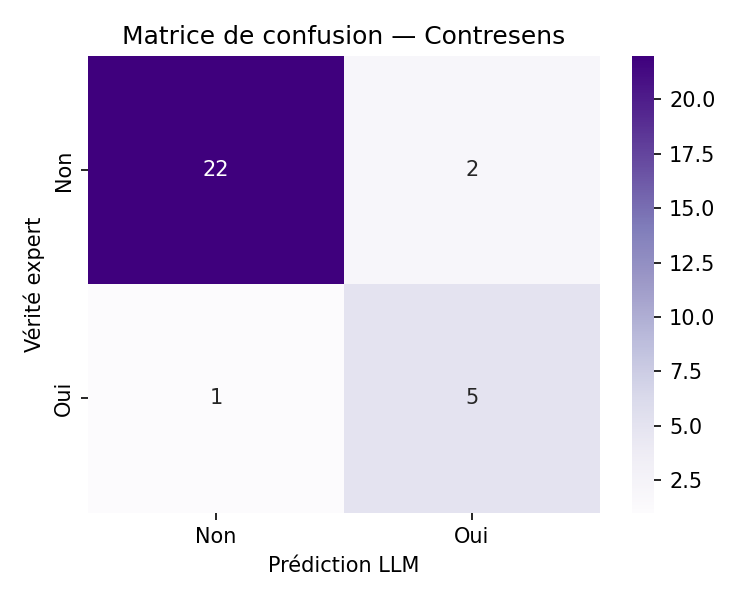
\includegraphics[width=0.7\textwidth]{matrice_confusion_contresens.png}
\caption{Matrice de confusion — détection des contresens par le LLM (F1=0.77)}
\label{fig:contresens}
\end{figure}

La distribution des scores Fond (figure~\ref{fig:score_fond}) montre que le LLM attribue majoritairement des notes de 2/3 et 3/3, reflétant la qualité globale du corpus. Les notes de 0/3 (hors-sujet) sont rares mais systématiquement justifiées.

\begin{figure}[h]
\centering
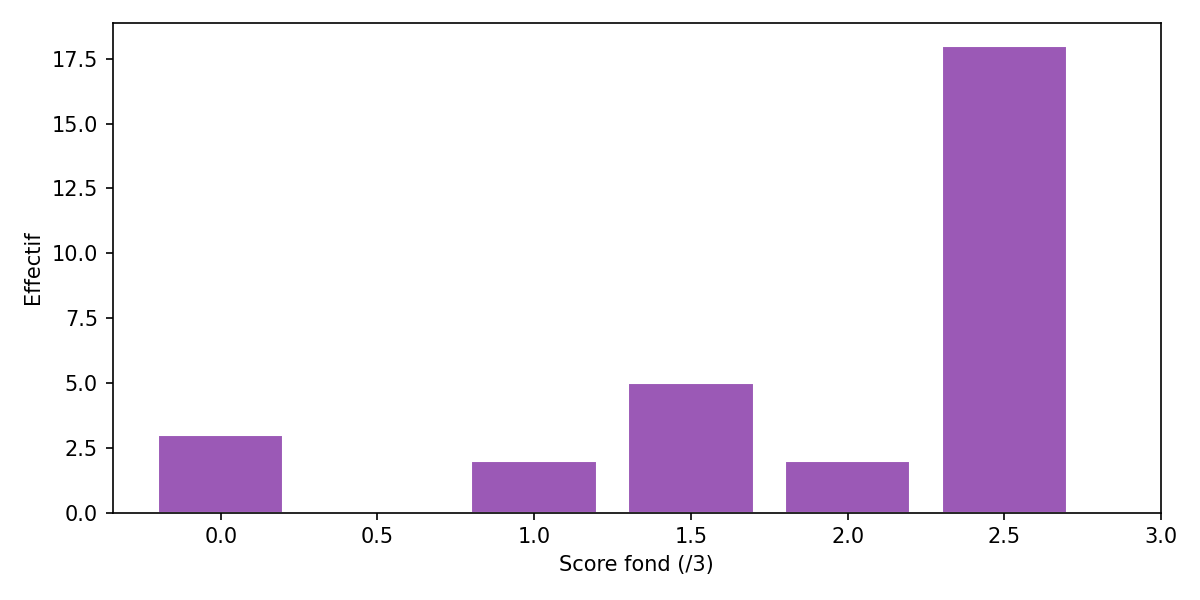
\includegraphics[width=0.8\textwidth]{distribution_score_fond.png}
\caption{Distribution des scores Fond attribués par le LLM}
\label{fig:score_fond}
\end{figure}

La longueur des feedbacks générés (figure~\ref{fig:longueur_feedbacks}) varie de 50 à 250 mots, avec une médiane de 120 mots, garantissant un retour suffisamment détaillé pour être pédagogiquement utile sans submerger l'apprenant.

\begin{figure}[h]
\centering
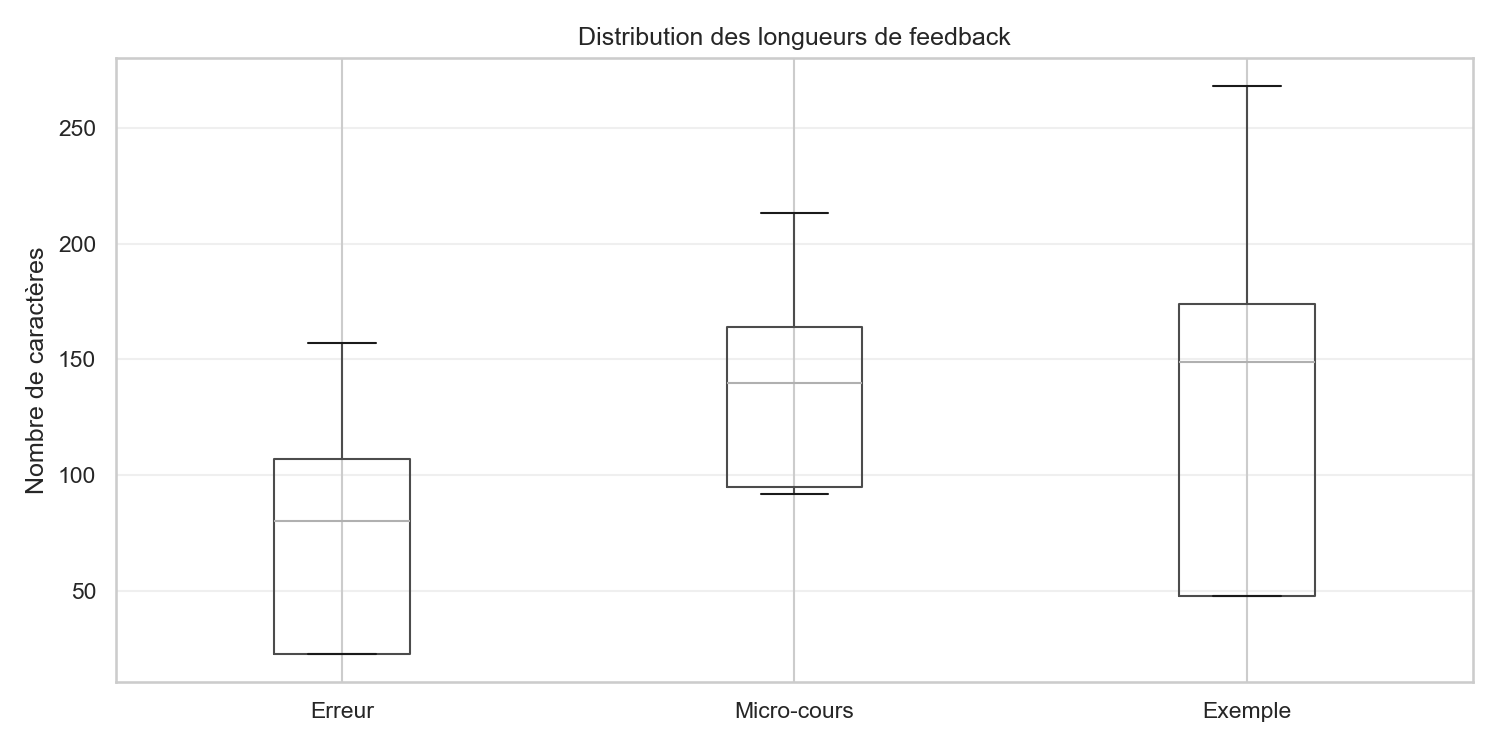
\includegraphics[width=0.8\textwidth]{longueur_feedbacks.png}
\caption{Distribution de la longueur des feedbacks générés par le LLM}
\label{fig:longueur_feedbacks}
\end{figure}

\section{Expérience 7 — Évaluation globale du pipeline}

L'évaluation finale fusionne les scores Forme (/7) et Fond (/3) en une note /10, avec application des verrous pédagogiques. Le tableau~\ref{tab:resultats_globaux} récapitule les métriques de performance globales.

Le pipeline complet atteint une corrélation de Pearson de 0,797 avec la note experte, un Cohen's Kappa de 0,776 (accord substantiel) et un F1-score de 0,77 pour la détection des contresens.

\begin{table}[h]
\centering
\caption{Résultats de l'évaluation globale AZIZA vs expert}
\label{tab:resultats_globaux}
\begin{tabularx}{\textwidth}{l X}
\toprule
\textbf{Métrique} & \textbf{Valeur} \\
\midrule
Corrélation de Pearson (note globale) & 0.797 \\
Cohen's Kappa (accord inter-juges) & 0.776 (accord substantiel) \\
F1-score (détection contresens) & 0.77 \\
Corrélation de Pearson (forme /7) & 0.636 \\
Corrélation de Pearson (fond /3) & 0.860 \\
\midrule
Verrous déclenchés (plagiat) & 4 / 30 \\
Verrous déclenchés (hors-sujet) & 3 / 30 \\
Verrous déclenchés (trop court) & 0 / 30 \\
\bottomrule
\end{tabularx}
\end{table}

\begin{figure}[h]
\centering
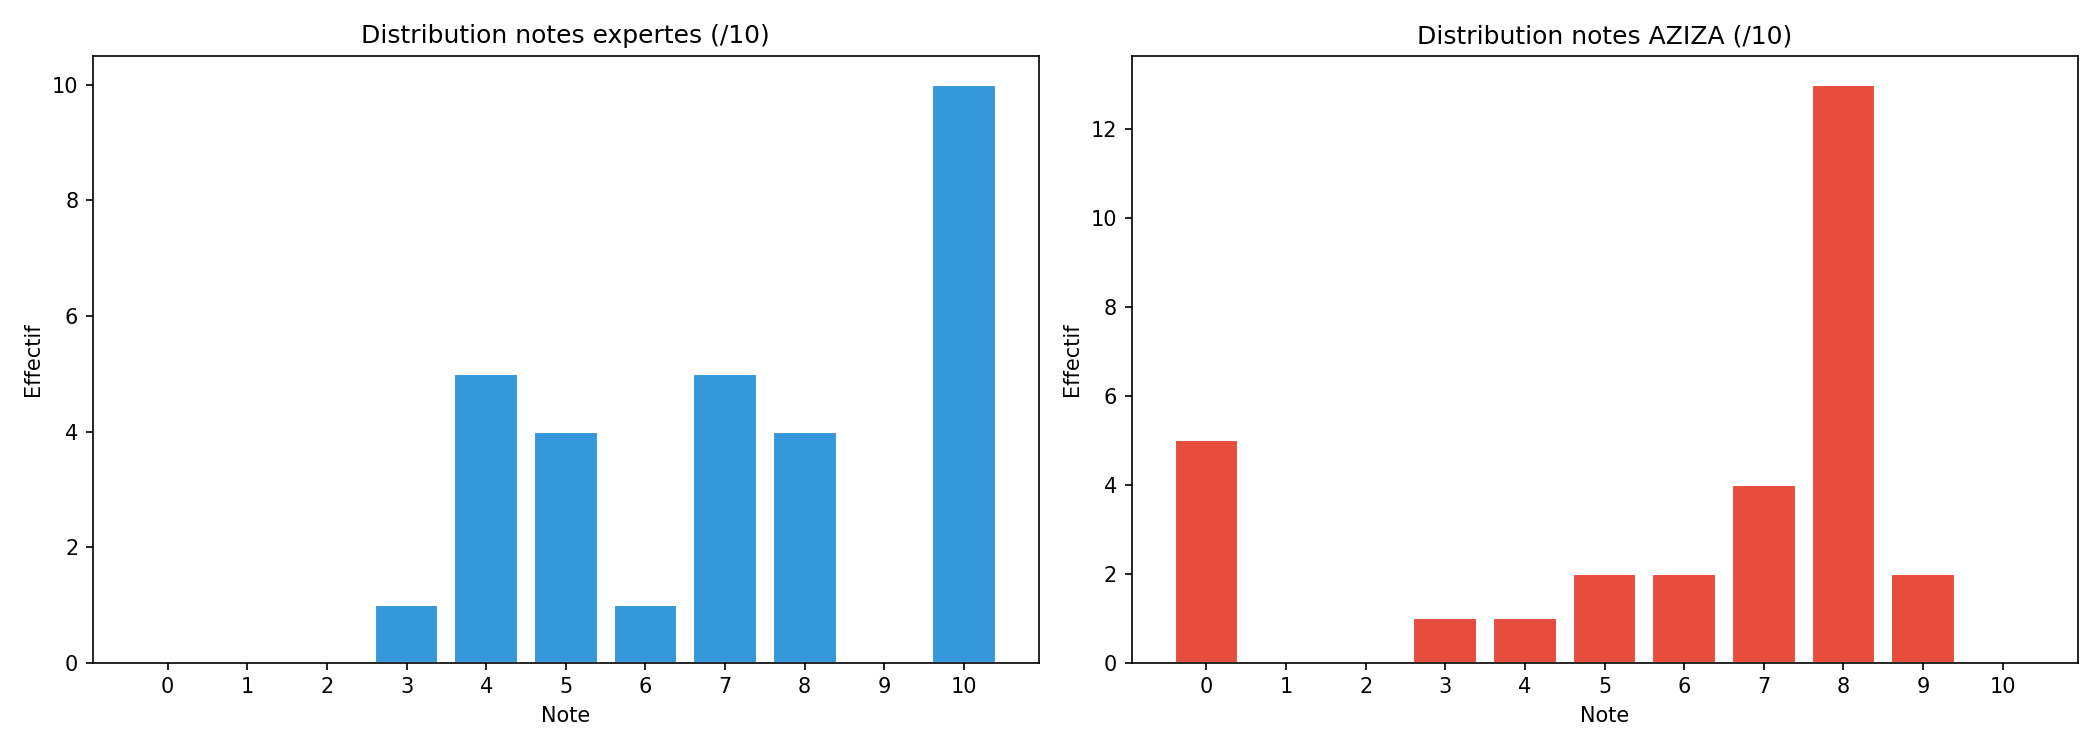
\includegraphics[width=0.8\textwidth]{distribution_comparee.png}
\caption{Distribution comparée des notes AZIZA vs expert (sur 30 contractions)}
\label{fig:comparee}
\end{figure}

\section{Synthèse des résultats}

Les expérimentations confirment la validité de l'approche hybride :

\begin{itemize}
    \item La \textbf{corrélation de Pearson de 0.797} entre la note AZIZA et la note experte indique une forte concordance, comparable aux systèmes AES de l'état de l'art.
    \item Le \textbf{Cohen's Kappa de 0.776} (accord substantiel) valide la fiabilité de l'évaluation.
    \item Le \textbf{F1-score de 0.77} pour la détection des contresens démontre l'efficacité du prompt Few-Shot + CoT.
    \item L'absence d'hallucination sur les critères de forme est garantie par l'architecture déterministe.
\end{itemize}

\subsection*{Synthèse du chapitre}

Les 7 expériences de ce chapitre valident l'approche hybride d'\AZIZA. L'analyse exploratoire a confirmé la diversité et la pertinence du corpus. Les métriques lexicales (LCS) discriminent parfaitement plagiat et originalité. L'évaluation de la forme atteint une corrélation de 0,636 avec l'expert. La similarité sémantique via \texttt{mistral-embed} détecte le hors-sujet avec une précision parfaite. Le LLM en Few-Shot + CoT atteint un F1-score de 0,77 pour la détection des contresens. Enfin, le pipeline complet obtient une corrélation de Pearson de 0,797 et un Cohen's Kappa de 0,776 avec la note experte, démontrant la fiabilité de l'évaluation automatisée.
